\chapter{Xây dựng giao thức xử lý}

\section{Tổng hợp và chuẩn hóa ngân hàng câu hỏi chương Tổ hợp – Xác suất lớp 11}
Phần này tiến hành tổng hợp và chuẩn hóa ngân hàng câu hỏi trắc nghiệm chương Tổ hợp – Xác suất lớp 11 dựa trên các nội dung cơ bản trong SGK Đại số và giải tích 11 (ban cơ bản): \textit{Quy tắc đếm} (bài 1), \textit{Hoán vị, tổ hợp, chỉnh hợp} (HV, TH, CH) (bài 2), \textit{Nhị thức Newton} (bài 3) và \textit{Xác suất của biến cố} (bài 4, 5).\par
Để sử dụng được ngân hàng câu hỏi cho việc đánh giá riêng lẻ từng học sinh theo \textit{lý thuyết ứng đáp câu hỏi} (IRT), cần có một ngân hàng câu hỏi đã chuẩn hóa sẵn theo các tham số \textit{độ khó} ($b$) và \textit{độ phân biệt} ($a$) – là những tham số độc lập so với mẫu. Phần lớn các câu hỏi trong luận văn này được tổng hợp từ \cite{luyen2018xay} và \cite{truc2018xay}. Trong đó có 44 câu hỏi có thể sử dụng ngay (đã được thực nghiệm và phân tích bằng IATA) có số lượng cụ thể như sau:\par

\begin{longtable}{SlScScScScSc}
	\multicolumn{1}{Sc}{\textbf{Chủ đề}} & \textbf{Mức độ 1} & \textbf{Mức độ 2} & \textbf{Mức độ 3} & \textbf{Mức độ 4} & \textbf{Tổng cộng}\\\hline\endhead\hline\endfoot
	Quy tắc đếm     & $2$ & $-$  & $3$  & $-$ & $5$  \\
	HV, TH, CH      & $-$ & $4$  & $1$  & $-$ & $5$  \\
	Nhị thức Newton & $5$ & $7$  & $9$  & $2$ & $23$ \\
	Xác suất        & $1$ & $7$  & $2$  & $1$ & $11$ \\\hline
	\textbf{Tổng cộng} & $8$ & $18$ & $15$ & $3$ & $44$ \\
\end{longtable}\par

\noindent\textbf{Câu hỏi trắc nghiệm phần \textit{Quy tắc đếm}:}
\begin{enumerate}[label=\textbf{Câu \arabic*.},align=left,left=0cm..0cm,itemindent=*]
	% Quy tắc đếm
	\item Mỗi ngày T đều đi từ nhà (vị trí $A$) tới trường (vị trí $D$) được nối với nhau như hình vẽ bên dưới. T có bao nhiêu con đường có thể đi và không đi qua một vị trí 2 lần?\par {\centering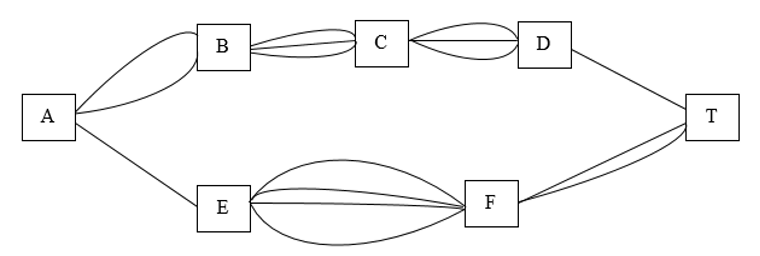
\includegraphics[width=9cm]{item-illustrations/G1-Q9}\par}
	\begin{multicols}{4}\begin{enumerate}[label=\textbf{\Alph*.},align=left,left=1cm..0cm,itemindent=*]
		\item $26$. \item $144$. \item $16$. \item $63$.
	\end{enumerate}\end{multicols}
	\item Kỷ niệm 77 năm ngày thành lập Đoàn TNCS Hồ Chí Minh (26/3/1931 – 26/3/2008), Sở giáo dục đào tạo Thừa Thiên Huế tổ chức giải bóng đá học sinh THPT và có 16 trường đăng ký tham gia đá theo 3 vòng gồm 4 bảng A, B, C, D, mỗi bảng gồm 4 đội cách thức thi đấu như sau:\par
	– Vòng 1: Mỗi đội tuyển trong cùng một bản gặp nhau một lần và gặp tất cả các đội có trong bảng (ví dụ bảng A đội thứ nhất phải thi đấu với 3 đội còn lại).\par
	– Vòng 2 (bán kết):\par
	~~~~ Nhất A gặp nhất C.\par
	~~~~ Nhất B gặp nhất D.\par
	– Vòng 3 (chung kết):\par
	~~~~ Tranh giải 3: hai đội thua bán kết.\par
	~~~~ Tranh giải nhất: hai đội thắng bán kết.\par
	Giải bóng được tổ chức vào các ngày liên tiếp, mỗi ngày 4 trận. Hỏi ban tổ chức cần mượn sân vân động trong bao nhiêu ngày?
	\begin{multicols}{4}\begin{enumerate}[label=\textbf{\Alph*.},align=left,left=1cm..0cm,itemindent=*]
		\item $25$. \item $13$. \item $7$. \item $12$.
	\end{enumerate}\end{multicols}
	\item Cho 2 tập hợp $A=\{1;2;3;4;5\}$ và $B=\{7;8;9\}$. Có bao nhiêu số có 2 chữ số $\overline{ab}$ với $a\in A$ và $b\in B$.
	\begin{multicols}{4}\begin{enumerate}[label=\textbf{\Alph*.},align=left,left=1cm..0cm,itemindent=*]
		\item 8 số. \item 10 số. \item 15 số. \item 30 số.
	\end{enumerate}\end{multicols}
	\item Một cuộc thi chạy đua 100m gồm 5 người có ba giải thưởng là nhất, nhì và ba. Có bao nhiêu khả năng nhận giải thưởng từ 5 người chơi?
	\begin{enumerate}[label=\textbf{\Alph*.},align=left,left=1cm..0cm,itemindent=*]
		\item 10 khả năng. \item 60 khả năng. \item 120 khả năng. \item 6 khả năng.
	\end{enumerate}
	\item Một cặp vợ chồng đều có kiểu gen dị hợp. Có bao nhiêu kiểu gen ở đời con?
	\begin{multicols}{4}\begin{enumerate}[label=\textbf{\Alph*.},align=left,left=1cm..0cm,itemindent=*]
		\item 3 kiểu. \item 4 kiểu. \item 5 kiểu. \item 6 kiểu.
	\end{enumerate}\end{multicols}
\end{enumerate}\par

\noindent\textbf{Đáp án và các tham số:}
\begin{longtable}{SlScScSrSr}
	\multicolumn{1}{Sc}{\textbf{Câu hỏi}} & \textbf{Mức độ} & \textbf{Đáp án} & \multicolumn{1}{Sc}{$a$} & \multicolumn{1}{Sc}{$b$}\\\hline\endhead\hline\endfoot
	Câu 1 & 3 & D & $2.93$ & $-0.09$\\
	Câu 2 & 3 & C & $1.34$ & $-0.18$\\
	Câu 3 & 1 & C & $1.69$ & $-0.31$\\
	Câu 4 & 1 & B & $1.85$ & $-0.33$\\
	Câu 5 & 3 & B & $1.40$ & $-0.60$\\
\end{longtable}

\noindent\textbf{Câu hỏi trắc nghiệm phần \textit{Hoán vị, tổ hợp, chỉnh hợp}:}\par
\begin{enumerate}[label=\textbf{Câu \arabic*.},align=left,left=0cm..0cm,itemindent=*]
	% Hoán vị, tổ hợp, chỉnh hợp
	\item Cho 2 đường thẳng $a$ và $b$ song song nhau. Trên $a$ lấy 5 điểm phân biệt, trên $b$ lấy 10 điểm phân biệt. Có thể tạo nên bao nhiêu tam giác có các đỉnh là các điểm nằm trên $a$ và $b$?
	\begin{enumerate}[label=\textbf{\Alph*.},align=left,left=1cm..0cm,itemindent=*]
		\item 325 tam giác. \item 425 tam giác. \item 225 tam giác. \item 100 tam giác.
	\end{enumerate}
	\item Một đội xây dựng gồm 3 kỹ sư, 7 công nhân lập thành một tổ công tác thành 5 người. Hỏi có bao nhiêu cách lập được một tổ công tác gồm 1 kỹ sư làm tổ trưởng, 1 công nhân làm tổ phó và 3 công nhân tổ viên.
	\begin{multicols}{4}\begin{enumerate}[label=\textbf{\Alph*.},align=left,left=1cm..0cm,itemindent=*]
		\item $735$. \item $105$. \item $240$. \item $420$.
	\end{enumerate}\end{multicols}
	\item Cho mạch điện sau:\par
	{\centering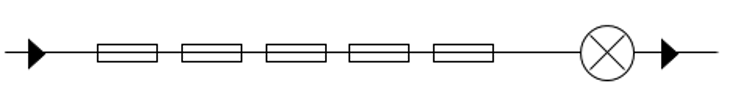
\includegraphics[width=10cm]{item-illustrations/G1-Q43}\par}
	Với 5 cầu chỉ mắc nối tiếp trước một bóng đèn. Có nhiêu trường hợp dòng điện không thể truyền đến bóng đèn?
	\begin{enumerate}[label=\textbf{\Alph*.},align=left,left=1cm..0cm,itemindent=*]
		\item 5 trường hợp. \item 120 trường hợp. \item 325 trường hợp. \item 31 trường hợp.
	\end{enumerate}
	\item Tìm số nguyên dương $n$ thỏa điều kiện $A_{n}^{2}-3C_{n}^{2}=15-5n$.
	\begin{enumerate}[label=\textbf{\Alph*.},align=left,left=1cm..0cm,itemindent=*]
		\item $\left[ \begin{array}{l} n=5\\ n=6\\ n=12 \end{array} \right.$.
		\item $\left[ \begin{array}{l} n=5\\ n=6 \end{array} \right.$.
		\item $n=5$.
		\item $n=6$.
	\end{enumerate}
	\item Cần chọn ra một nhóm 3 người trong 7 người để tham gia lao động. Có bao nhiêu cách chọn?
	\begin{multicols}{4}\begin{enumerate}[label=\textbf{\Alph*.},align=left,left=1cm..0cm,itemindent=*]
		\item $210$. \item $21$. \item $10$. \item $35$.
	\end{enumerate}\end{multicols}
\end{enumerate}\par

\noindent\textbf{Đáp án và các tham số:}
\begin{longtable}{SlScScSrSr}
	\multicolumn{1}{Sc}{\textbf{Câu hỏi}} & \textbf{Mức độ} & \textbf{Đáp án} & \multicolumn{1}{Sc}{$a$} & \multicolumn{1}{Sc}{$b$}\\\hline\endhead\hline\endfoot
	Câu 1 & 2 & A & $1.17$ & $-0.39$\\
	Câu 2 & 2 & D & $0.96$ & $-0.81$\\
	Câu 3 & 3 & D & $2.53$ & $0.31$ \\
	Câu 4 & 2 & B & $1.09$ & $-0.62$\\
	Câu 5 & 2 & D & $0.89$ & $-1.33$\\
\end{longtable}\par

\noindent\textbf{Câu hỏi trắc nghiệm phần \textit{Nhị thức Newton}:}\par
\begin{enumerate}[label=\textbf{Câu \arabic*.},align=left,left=0cm..0cm,itemindent=*]
	% Nhị thức Newton
	\item Cho khai triển $\left(x^3+2x^2+1\right)^{10}=a_1+a_2x+a_3x^2+...+a_{20}x^{20}$. Tính tổng $$S=a_1+2a_2+4a_3+...+2^{20}a_{20}.$$
	\begin{multicols}{4}\begin{enumerate}[label=\textbf{\Alph*.},align=left,left=1cm..0cm,itemindent=*]
		\item $S=15^{10}$. \item $S=17^{10}$. \item $S=17^{20}$. \item $S=7^{10}$.
	\end{enumerate}\end{multicols}
	\item Trong khai triển $(1-x)^{12}$, hệ số đứng trước $x^7$ là
	\begin{multicols}{4}\begin{enumerate}[label=\textbf{\Alph*.},align=left,left=1cm..0cm,itemindent=*]
		\item $330$. \item $-33$. \item $-72$. \item $-792$.
	\end{enumerate}\end{multicols}
	\item Công thức khai triển của $(a+b)^n$ là
	\begin{enumerate}[label=\textbf{\Alph*.},align=left,left=1cm..0cm,itemindent=*]
		\item $\sum_{k=1}^nC_n^ka^{n+k}b^k$. \item $\sum_{k=0}^nC_n^ka^{n-k}b^k$. \item $\sum_{k=1}^nC_n^ka^{n-k}b^k$. \item $\sum_{k=0}^nC_n^ka^{n+k}b^k$.
	\end{enumerate}
	\item Mệnh đề nào sau đây là đúng?
	\begin{enumerate}[label=\textbf{\Alph*.},align=left,left=1cm..0cm,itemindent=*]
		\item $(a-b)^n=\sum_{k=0}^nC_n^ka^{n-k}b^k$, ($a,b\in\mathbb{R}$, $n\in\mathbb{N}^{*}$).
		\item $(a-b)^n=\sum_{k=0}^n(-1)C_n^ka^{n-k}b^k$, ($a,b\in\mathbb{R}$, $n\in\mathbb{N}^{*}$).
		\item $0^n=C_n^0+C_n^1+C_n^2+C_n^3+\ldots+C_n^n$, ($n\in\mathbb{N}^{*}$).
		\item $2^n=C_n^0-C_n^1+C_n^2-C_n^3+\ldots+C_n^n$, ($n\in\mathbb{N}^{*}$).
	\end{enumerate}
	\item Trong khai triển $(a+b)^n$, ($a,b\in\mathbb{R}$, $n\in\mathbb{N}^{*}$). Tổng các số mũ của $a$ và $b$ trong mỗi số hạng bằng
	\begin{multicols}{4}\begin{enumerate}[label=\textbf{\Alph*.},align=left,left=1cm..0cm,itemindent=*]
		\item $n+1$. \item $2n$. \item $n$. \item $2n+1$.
	\end{enumerate}\end{multicols}
	\item Trong khai triển $(a+b)^n$, ($a,b\in\mathbb{R}$, $n\in\mathbb{N}^{*}$), ta được bao nhiêu số hạng?
	\begin{enumerate}[label=\textbf{\Alph*.},align=left,left=1cm..0cm,itemindent=*]
		\item $n+1$ số hạng. \item $2n$ số hạng. \item $n$ số hạng. \item $2n+1$ số hạng.
	\end{enumerate}
	\item Số hạng tổng quát của khai triển $(a+b)^n$, ($a,b\in\mathbb{R}$, $n\in\mathbb{N}^{*}$) là
	\begin{enumerate}[label=\textbf{\Alph*.},align=left,left=1cm..0cm,itemindent=*]
		\item $T_{k-1}=C_n^ka^{n-k}b^k$. \item $T_{k-1}=C_n^ka^{n+k}b^k$. \item $T_{k+1}=C_n^ka^{n-k}b^k$. \item $T_{k+1}=C_n^ka^{n+k}b^k$.
	\end{enumerate}
	\item Tính tổng $S=2^{13}C_{13}^0-2^{12}.3^1C_{13}^1+2^{11}.3^2C_{13}^2-2^{10}.3^3C_{13}^3+...+3^{13}C_{13}^{13}$.
	\begin{multicols}{4}\begin{enumerate}[label=\textbf{\Alph*.},align=left,left=1cm..0cm,itemindent=*]
		\item $(-1)^{13}$. \item $5^{13}$. \item $(-5)^{13}$. \item $1^{13}$.
	\end{enumerate}\end{multicols}
	\item Nhị thức $(5+x^2)^{12}$ có khai triển là
	\begin{enumerate}[label=\textbf{\Alph*.},align=left,left=1cm..0cm,itemindent=*]
		\item $5^{12}C_{12}^0-5^{11}xC_{12}^1+...+(-1)x^{24}C_{12}^{12}$.
		\item $5^{12}C_{12}^0-5^{11}x^2C_{12}^1+...+ \left(-1\right) x^{24}C_{12}^{12}$.
		\item $5^{12}C_{12}^0+5^{11}x^2C_{12}^1+...+x^{24}C_{12}^{12}$.
		\item $5^{12}C_{12}^0+5^{11}xC_{12}^1+...+x^{24}C_{12}^{12}$.
	\end{enumerate}
	\item Trong khai triển nhị thức $\left(x+y^2\right)^{10}$ thành đa thức và xếp theo thứ tự lũy thừa tăng dần của $x$ thì số hạng thứ 6 kể từ trái sang phải là bao nhiêu?
	\begin{multicols}{4}\begin{enumerate}[label=\textbf{\Alph*.},align=left,left=1cm..0cm,itemindent=*]
		\item $C_{10}^6x^4y^6$. \item $C_{10}^5x^5y^5$. \item $C_{10}^6x^4y^8$. \item $C_{10}^5x^5y^{10}$.
	\end{enumerate}\end{multicols}
	\item Trong khai triển $(2a-b)^5$, ($a,b\in\mathbb{R}$) hệ số của số hạng thứ 3 bằng
	\begin{multicols}{4}\begin{enumerate}[label=\textbf{\Alph*.},align=left,left=1cm..0cm,itemindent=*]
		\item $80$. \item $40$. \item $-80$. \item $-40$.
	\end{enumerate}\end{multicols}
	\item Khai triển nhị thức $(x+2)^{n+6}$, ($x\in\mathbb{R}$, $n\in\mathbb{N}$) có tất cả $17$ số hạng. Vậy $n$ bằng
	\begin{multicols}{4}\begin{enumerate}[label=\textbf{\Alph*.},align=left,left=1cm..0cm,itemindent=*]
		\item $10$. \item $11$. \item $12$. \item $17$.
	\end{enumerate}\end{multicols}
	\item Trong khai triển $\left(3x^2-y\right)^{10}$, hệ số của số hạng chính giữa là
	\begin{multicols}{4}\begin{enumerate}[label=\textbf{\Alph*.},align=left,left=1cm..0cm,itemindent=*]
		\item $-3^4C_{10}^4$. \item $3^4C_{10}^4$. \item $-3^5C_{10}^5$. \item $3^5C_{10}^5$.
	\end{enumerate}\end{multicols}
	\item Cho hàm số $f(x)=x(x+1)^{2018}$. Tính $f'(1)$.
	\begin{enumerate}[label=\textbf{\Alph*.},align=left,left=1cm..0cm,itemindent=*]
		\item $f'(1)=2^{2018}+2^{2017}$.
		\item $f'(1)=2^{2018}+2018.2^{2017}$.
		\item $f'(1)=2^{2018}+2018.2^{2018}$.
		\item $f'(1)=2^{2017}+2018.2^{2017}$.
	\end{enumerate}
	\item Tìm số nguyên dương $n$ sao cho $C_n^0+2C_n^1+4C_n^2+...+2^nC_n^n=243$.
	\begin{multicols}{4}\begin{enumerate}[label=\textbf{\Alph*.},align=left,left=1cm..0cm,itemindent=*]
		\item $n=4$. \item $n=5$. \item $n=11$. \item $n=12$.
	\end{enumerate}\end{multicols}
	\item Cho khai triển $(2x-1)^4=a_0x^{14}+a_1x^{13}+...+a_{14}$. Tính tổng $$T=a_0-a_1+a_2-a_3+...+a_{14}.$$
	\begin{multicols}{4}\begin{enumerate}[label=\textbf{\Alph*.},align=left,left=1cm..0cm,itemindent=*]
		\item $T=1$. \item $T=3^4$. \item $T=-1$. \item $T=-3^4$.
	\end{enumerate}\end{multicols}
	\item Số nào sau đây không phải hệ số của $x^8$ trong khai triển $(1+x)^{10}$?
	\begin{multicols}{4}\begin{enumerate}[label=\textbf{\Alph*.},align=left,left=1cm..0cm,itemindent=*]
		\item $C_{10}^8-C_9^8$. \item $C_{10}^2$. \item $C_9^7+C_9^8$. \item $C_{10}^8$.
	\end{enumerate}\end{multicols}
	\item Cho khai triển $(x-2)^{100}=a_0+a_1x+a_2x^2+...+a_{100}x^{100}$. Hệ số $a_{97}$ là
	\begin{multicols}{4}\begin{enumerate}[label=\textbf{\Alph*.},align=left,left=1cm..0cm,itemindent=*]
		\item $-2^3C_{100}^3$. \item $-2^{97}C_{100}^{97}$. \item $2^3C_{100}^3$. \item $2^{97}C_{100}^{97}$.
	\end{enumerate}\end{multicols}
	\item Tìm giá trị nguyên dương $n$, biết $T=C_{2n}^0+C_{2n}^1+C_{2n}^2+...+C_{2n}^{2n}=1024$.
	\begin{multicols}{4}\begin{enumerate}[label=\textbf{\Alph*.},align=left,left=1cm..0cm,itemindent=*]
		\item $n=1$. \item $n=2$. \item $n=5$. \item $n=10$.
	\end{enumerate}\end{multicols}
	\item Tính tổng $S=n.3^0C_n^n+(n-1).3^1C_n^{n-1}+(n-2).3^2C_n^{n-2}+...+1.3^{n-1}C_n^1$.
	\begin{enumerate}[label=\textbf{\Alph*.},align=left,left=1cm..0cm,itemindent=*]
		\item $S=n.4^{n-1}$. \item $S=n.4^n$. \item $S=n.3^n$. \item $S=n.3^{n-1}$.
	\end{enumerate}
	\item Tìm số nguyên dương $n$ thỏa $$C_{2n-1}^1-2.2C_{2n-1}^2-3.2C_{2n-1}^3+...-(2n-1)x^{2n-2}C_{2n-1}^{2n-1}=2017.$$
	\begin{enumerate}[label=\textbf{\Alph*.},align=left,left=1cm..0cm,itemindent=*]
		\item $n=1008$. \item $n=1009$. \item $n=-1008$. \item $n=-1009$.
	\end{enumerate}
	\item Tìm hệ số lớn nhất của khai triển $(1+x)^n$. Biết rằng tổng tất cả các hệ số là $4096$.
	\begin{multicols}{4}\begin{enumerate}[label=\textbf{\Alph*.},align=left,left=1cm..0cm,itemindent=*]
		\item $0$. \item $1$. \item $C_{12}^5$. \item $C_{12}^6$.
	\end{enumerate}\end{multicols}
	\item Tính tổng $S=1.2^0C_{n+2}^1+2.2^1C_{n+2}^2+3.2^2C_{n+2}^3+...+(n+2).2^{n+1}C_{n+2}^{n+2}$.
	\begin{enumerate}[label=\textbf{\Alph*.},align=left,left=1cm..0cm,itemindent=*]
		\item $(n+2).3^{n+2}$. \item $(n+2).3^{n+1}$. \item $(n+2).2^{n+2}$. \item $(n+2).2^{n+1}$.
	\end{enumerate}
\end{enumerate}\par

\noindent\textbf{Đáp án và các tham số:}
\begin{longtable}{SlScScSrSr}
	\multicolumn{1}{Sc}{\textbf{Câu hỏi}} & \textbf{Mức độ} & \textbf{Đáp án} & \multicolumn{1}{Sc}{$a$} & \multicolumn{1}{Sc}{$b$} \\\hline\endhead\hline\endfoot
	Câu 1  & 3 & B & $0.21$ & \multicolumn{1}{Sc}{$-$} \\
	Câu 2  & 3 & D & $1.74$ & $-1.28$ \\
	Câu 3  & 1 & B & $1.31$ & $-1.18$ \\
	Câu 4  & 1 & B & $0.36$ & $-1.73$ \\
	Câu 5  & 1 & C & $0.78$ & $-0.67$ \\
	Câu 6  & 1 & A & $0.53$ & $-2.09$ \\
	Câu 7  & 1 & C & $0.81$ & $-1.34$ \\
	Câu 8  & 2 & A & $1.26$ & $-0.40$ \\
	Câu 9  & 2 & C & $0.17$ & $0.17$  \\
	Câu 10 & 2 & D & $0.74$ & $-0.99$ \\
	Câu 11 & 2 & A & $0.30$ & $0.41$  \\
	Câu 12 & 2 & A & $1.57$ & $-0.94$ \\
	Câu 13 & 2 & C & $1.06$ & $-0.98$ \\
	Câu 14 & 2 & B & $1.28$ & $-1.49$ \\
	Câu 15 & 3 & B & $0.33$ & $-2.25$ \\
	Câu 16 & 3 & B & $0.29$ & $0.54$  \\
	Câu 17 & 3 & A & $1.32$ & $-0.52$ \\
	Câu 18 & 3 & A & $1.66$ & $-0.60$ \\
	Câu 19 & 3 & C & $0.33$ & $0.48$  \\
	Câu 20 & 3 & A & $0.50$ & $0.41$  \\
	Câu 21 & 3 & C & $0.46$ & $0.90$  \\
	Câu 22 & 4 & D & $0.37$ & $-0.61$ \\
	Câu 23 & 4 & B & $0.17$ & $1.06$  \\
\end{longtable}\par

\noindent\textbf{Câu hỏi trắc nghiệm phần \textit{Xác suất}:}
\begin{enumerate}[label=\textbf{Câu \arabic*.},align=left,left=0cm..0cm,itemindent=*]
	\item Một nông dân có 8 con trâu. Hôm nay ông dắt theo 2 con để ra ruộng nhưng ông không biết rằng trong số trâu đó có 3 bị bệnh. Tính xác suất để cả 2 con trâu người nông dân chọn đều không bị bệnh.
	\begin{multicols}{4}\begin{enumerate}[label=\textbf{\Alph*.},align=left,left=1cm..0cm,itemindent=*]
		\item $P=\frac 5{14}$. \item $P=\frac 5{28}$. \item $P=\frac{25}{28}$. \item $P=\frac 3{28}$.
	\end{enumerate}\end{multicols}
	\item Một khối lập phương có tất cả được sơn màu và được chia thành 125 khối nhỏ bằng nhau bởi các mặt phẳng song song với các mặt của khối lập phương (hình vẽ).\par
	{\centering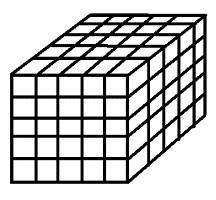
\includegraphics[width=4cm]{item-illustrations/G2-Q30}\par}
	Lấy ngẫu nhiên 15 khối nhỏ. Xác suất để lấy được 6 khối nhỏ sơn đúng 1 mặt gần bằng
	\begin{multicols}{4}\begin{enumerate}[label=\textbf{\Alph*.},align=left,left=1cm..0cm,itemindent=*]
		\item $0,00004$. \item $0,237$. \item $0,212$. \item $0,191$.
	\end{enumerate}\end{multicols}
	\item Lớp có 30 học sinh trong đó có 10 học sinh cận thị. Người ta lần lượt kiểm tra ngẫu nhiên từng học sinh cho đến khi phát hiện một học sinh cận thị thì dừng lại. Xác suất để kiểm tra tới học sinh thứ 5 thì ngừng lại (kiểm tra có hoàn lại) là
	\begin{multicols}{4}\begin{enumerate}[label=\textbf{\Alph*.},align=left,left=1cm..0cm,itemindent=*]
		\item $0,068$. \item $0,067$. \item $0,066$. \item $0,065$.
	\end{enumerate}\end{multicols}
	\item Một lớp 30 học sinh. Chọn ngẫu nhiên 3 học sinh để tham gia hoạt động của Đoàn trường. Xác suất để chọn được 2 nam và 1 nữ là $\frac{54}{1015}$. Tính số học sinh nữ của lớp.
	\begin{multicols}{4}\begin{enumerate}[label=\textbf{\Alph*.},align=left,left=1cm..0cm,itemindent=*]
		\item $18$. \item $15$. \item $12$. \item $9$.
	\end{enumerate}\end{multicols}
	\item Thả rơi một chất điểm vào một tấm bìa hình chữ nhật có chiều dài và chiều rộng lần lượt là 25 và 10 (cm). Một điểm $A$ cố định được vẽ trên tấm bìa như hình vẽ. Tính xác suất để chất điểm cách điểm $A$ từ 3 đến 4 (cm).\par
	{\centering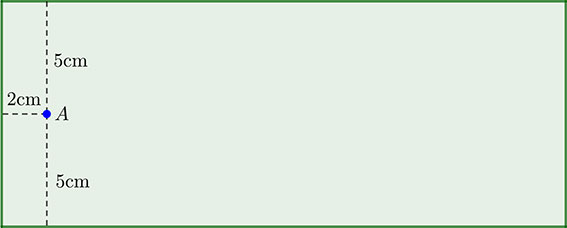
\includegraphics[width=10cm]{item-illustrations/G2-Q58}\par}
	\begin{enumerate}[label=\textbf{\Alph*.},align=left,left=1cm..0cm,itemindent=*]
		\item $P=0,049$. \item $P=0,044$. \item $P=0,061$. \item $P=0,088$.
	\end{enumerate}
	\item Ở người có một gen b gây bệnh bạch tạng lặn hoàn toàn so với gen B qui định màu da bình thường. Một đôi vợ chồng đều có gen đều dạng dị hợp (tức là có chứa một gen lặn). Tính xác suất để họ sinh được 5 đứa con thì 2 con trai bình thường, 2 con gái bình thường và 1 con trai bị bệnh.
	\begin{enumerate}[label=\textbf{\Alph*.},align=left,left=1cm..0cm,itemindent=*]
		\item $P=0,002$. \item $P=0,074$. \item $P=0,003$. \item $P=0,084$.
	\end{enumerate}
	\item Lỗi chính tả của một học sinh lớp 2 trên mỗi trang vở là đại lượng ngẫu nhiên $X$ có bảng phân phối xác suất như sau:
	\begin{longtable}{|c|c|c|c|c|c|c|}\hline
	$X$ & 0   & 1   & 2   & 3 	& 4 	& 5   \\\hline
	$P$ & 0,3 & 0,3 & 0,2 & 0,01 & 0,09 & 0,1 \\\hline
	\end{longtable}
	Tính xác suất để mỗi trang sai ít nhất 3 lỗi.
	\begin{enumerate}[label=\textbf{\Alph*.},align=left,left=1cm..0cm,itemindent=*]
		\item $P=0,2$. \item $P=0,3$. \item $P=0,29$. \item $P=0,009$.
	\end{enumerate}
	\item Lợi nhuận (tỷ đồng) hai dự án $A$ và $B$, ký hiệu $X_A$ và $X_B$ có bảng phân phối xác suất như sau:
	\begin{longtable}{|c|c|c|c|}\hline
	$X_A$ & $-2$ & 3   & 10  \\\hline
	$P$   & 0.2  & 0.6 & 0.2 \\\hline\hline
	$X_B$ & 1 	& 4   & 9   \\\hline
	$P$   & 0.4  & 0.4 & 0.2 \\\hline
	\end{longtable}
	Tìm lợi nhuận trung bình của mỗi dự án và dự án nào có độ ổn định cao hơn?
	\begin{enumerate}[label=\textbf{\Alph*.},align=left,left=1cm..0cm,itemindent=*]
		\item $E\left( {{X}_{A}} \right)=3,4; E\left( {{X}_{B}} \right)=3,3$ và dự án $A$ ổn định hơn.
		\item $E\left( {{X}_{A}} \right)=3,4; E\left( {{X}_{B}} \right)=3,3$ và dự án $B$ ổn định hơn.
		\item $E\left( {{X}_{A}} \right)=3,3; E\left( {{X}_{B}} \right)=3,4$ và dự án $A$ ổn định hơn.
		\item $E\left( {{X}_{A}} \right)=3,3; E\left( {{X}_{B}} \right)=3,4$ và dự án $B$ ổn định hơn.
	\end{enumerate}
	\item Khảo sát trên 100 sinh viên về thời gian sử dụng máy tính trong một ngày thu được biểu đồ sau:\par
	{\centering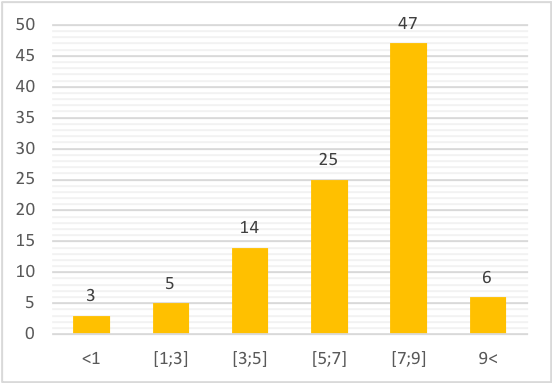
\includegraphics[width=7cm]{item-illustrations/G2-Q127}\par}
	Gọi $X$ là đại lượng thời gian sử dụng máy tính (giờ). Tính $P\left( 5,28\leqslant X<9 \right)$.
	\begin{enumerate}[label=\textbf{\Alph*.},align=left,left=1cm..0cm,itemindent=*]
		\item $P\left( 5,28\leqslant X<9,2 \right)=0,78$.
		\item $P\left( 5,28\leqslant X<9,2 \right)=0,47$.
		\item $P\left( 5,28\leqslant X<9,2 \right)=0,72$.
		\item $P\left( 5,28\leqslant X<9,2 \right)=0,53$.
	\end{enumerate}
	\item Một người đi bộ từ công ty về đến nhà thì phát hiện rớt mất ví tiền. Anh ta chắc chắn rằng ví bị rơi trên đoạn đường khoảng 100m trước cửa công ty nên quay lại tìm. Tính xác suất anh ta tìm được ví biết quãng đường từ nhà đến công ty là 1,5km.
	\begin{multicols}{4}\begin{enumerate}[label=\textbf{\Alph*.},align=left,left=1cm..0cm,itemindent=*]
		\item $P=\frac 1{15}$. \item $P=\frac 3{200}$. \item $P=\frac {14}{15}$. \item $P=\frac 16$.
	\end{enumerate}\end{multicols}
	\item Số lượng cá (kg) một ngư dân bắt được mỗi ngày được thống kê trong bảng sau:
	\begin{longtable}{|l|c|c|c|c|c|c|}\hline
	$X$ (kg) & 0 	 & 1 	  & 2 	& 3 	  & 4 	  & 5 	 \\\hline
	Xác suất & 1,6\% & 12,6\% & 21\% & 34,7\% & 21,9\% & 8,2\% \\\hline
	\end{longtable}
	Tính xác suất để người này câu được nhiều nhất 2kg cá.
	\begin{enumerate}[label=\textbf{\Alph*.},align=left,left=1cm..0cm,itemindent=*]
		\item $P=0,04\%$. \item $P=35,2\%$. \item $P=0,21\%$. \item $P=0,352\%$.
	\end{enumerate}
\end{enumerate}\par

\noindent\textbf{Đáp án và các tham số:}
\begin{longtable}{SlScScSrSr}
	\multicolumn{1}{Sc}{\textbf{Câu hỏi}} & \textbf{Mức độ} & \textbf{Đáp án} & \multicolumn{1}{Sc}{$a$} & \multicolumn{1}{Sc}{$b$} \\\hline\endhead\hline\endfoot
	Câu 1  & 2 & A & $0.87$ & $-1.02$ \\
	Câu 2  & 2 & C & $1.33$ & $-0.75$ \\
	Câu 3  & 2 & A & $1.14$ & $-0.32$ \\
	Câu 4  & 2 & A & $1.59$ & $-0.35$ \\
	Câu 5  & 1 & B & $0.88$ & $0.04$  \\
	Câu 6  & 3 & D & $0.60$ & $-1.29$ \\
	Câu 7  & 4 & A & $0.78$ & $0.29$  \\
	Câu 8  & 2 & C & $0.84$ & $-0.32$ \\
	Câu 9  & 3 & B & $0.23$ & $1.02$  \\
	Câu 10 & 2 & A & $1.29$ & $-0.54$ \\
	Câu 11 & 2 & A & $1.33$ & $-0.84$ \\
\end{longtable}\par

Mục tiêu của cho ngân hàng câu hỏi chương Tổ hợp – Xác suất lớp 11 là khoảng 100 câu hỏi chia cho các chủ đề. Do đó, đề tài thực hiện thực nghiệm thêm 60 câu hỏi (được lựa chọn từ \cite{luyen2018xay} và \cite{truc2018xay}), có số lượng cụ thể như sau:\par
\begin{longtable}{SlScScScScSc}
	\multicolumn{1}{Sc}{\textbf{Chủ đề}} & \textbf{Mức độ 1} & \textbf{Mức độ 2} & \textbf{Mức độ 3} & \textbf{Mức độ 4} & \textbf{Tổng cộng}\\\hline\endhead\hline\endfoot
	Quy tắc đếm        & $4$  & $10$ & $5$  & $2$ & $21$ \\
	HV, TH, CH         & $7$  & $2$  & $7$  & $4$ & $20$ \\
	Nhị thức Newton    & $2$  & $-$  & $-$  & $-$ & $2$  \\
	Xác suất 	 	   & $6$  & $3$  & $5$  & $3$ & $17$ \\\hline
	\textbf{Tổng cộng} & $19$ & $15$ & $17$ & $9$ & $60$ \\
\end{longtable}\par

Trong đó, các câu hỏi được chia thành 02 đề độc lập nhau, mỗi đề gồm 30 câu hỏi:\par

\noindent\textbf{Đề thực nghiệm 1:}\par
\begin{enumerate}[label=\textbf{Câu \arabic*.},align=left,left=0cm..0cm,itemindent=*]
	\item Có bao nhiêu số tự nhiên có 3 chữ số
	\begin{multicols}{4}\begin{enumerate}[label=\textbf{\Alph*.},align=left,left=1cm..0cm,itemindent=*]
		\item $900$. \item $901$. \item $899$. \item $999$.
	\end{enumerate}\end{multicols}
	\item Bạn muốn mua một cây bút chì và một cây bút mực. Bút mực có 8 màu, bút chì cũng có 8 màu khác nhau. Vậy bạn có bao nhiêu cách lựa chọn?
	\begin{multicols}{4}\begin{enumerate}[label=\textbf{\Alph*.},align=left,left=1cm..0cm,itemindent=*]
		\item $64$ \item $32$ \item $20$ \item $16$
	\end{enumerate}\end{multicols}
	\item Cho tập hợp A có $n (n\geqslant 1)$ phần tử. Trong các phát biểu sau, phát biểu nào đúng?\par
	a) Số các hoán vị của A là $P_n=n!$.\par
	b) Khi sắp xếp n phần tử của A không theo một thứ tự, ta được một hoán vị.\par
	c) Số các hoán vị của A là $P_n=n(n-1)(n-2)...1$.\par
	d) Số nguyên $k$ ($1\leqslant k\leqslant n$). Mỗi tập con của $A$ có $k$ phần tử được gọi là một chỉnh hợp.\par
	e) Chỉnh hợp chập k của n phần tử của $A$ là khi ta lấy ra $k$ phần tử từ tập hợp và sắp xếp chúng theo một thứ tự.\par
	f) Quy tắc cộng mở rộng là $|A\cap B|=|A|+|B|+|A\cup B|.$
	\begin{multicols}{4}\begin{enumerate}[label=\textbf{\Alph*.},align=left,left=1cm..0cm,itemindent=*]
		\item a, c, e. \item a, b, d. \item b, e, f. \item b, c, d.
	\end{enumerate}\end{multicols}
	\item Cho tập hợp $A$ gồm có $n$ phần tử và một số nguyên $k$ thỏa mãn $1\leqslant k\leqslant n$. Mỗi tập hợp con gồm $k$ phần tử của $A$ được gọi là
	\begin{enumerate}[label=\textbf{\Alph*.},align=left,left=1cm..0cm,itemindent=*]
		\item Một chỉnh hợp chập $k$ của $n$ phần tử.
		\item Một tổ hợp chập $k$ của $n$ phần tử.
		\item Số chỉnh hợp chập $k$ của $n$ phần tử.
		\item Số tổ hợp chập $k$ của $n$ phần tử.
	\end{enumerate}
	\item Đẳng thức nào đúng?
	\begin{enumerate}[label=\textbf{\Alph*.},align=left,left=1cm..0cm,itemindent=*]
		\item $A_n^k=n.\left( n-1 \right)...\left( n-k-1 \right)$.
		\item $A_n^k=A_{n}^{n-k}$.
		\item $A_n^k=C_{n}^{k}.k!$.
		\item $A_n^k=C_{n}^{k}$.
	\end{enumerate}
	\item Phát biểu nào sau đây là \textbf{sai}?
	\begin{enumerate}[label=\textbf{\Alph*.},align=left,left=1cm..0cm,itemindent=*]
		\item Hai tổ hợp khác nhau thì có các phân tử khác nhau.
		\item Hai chỉnh hợp giống nhau khi có các phần tử giống nhau.
		\item Chỉnh hợp chập $n$ của $n$ phần tử chính là hoán vị của $n$ phần tử.
		\item Hai điểm $A$ và $B$ phân biệt thì $\overrightarrow{AB},\overrightarrow{BA}$ là các chỉnh hợp.
	\end{enumerate}
	\item Câu nào dưới đây \textbf{không đúng}?
	\begin{enumerate}[label=\textbf{\Alph*.},align=left,left=1cm..0cm,itemindent=*]
		\item $(a+b)^n=\sum_{k=0}^nC_n^ka^{n-k}b^k$.
		\item $(a+b)^n$ khi khai triển có $n$ số hạng.
		\item Tổng hệ số của $(a+b)^n$ khi khai triển là $2^n$.
		\item $C_n^p=C_n^q$ nếu $p+q=n$ hay $p=q$.
	\end{enumerate}
	\item Công thức $P(A.B)=P(A).P(B)$ đúng khi
	\begin{enumerate}[label=\textbf{\Alph*.},align=left,left=1cm..0cm,itemindent=*]
		\item Hai biến cố xung khắc.
		\item Hai biến cố đối.
		\item Hai biến cố độc lập.
		\item Hai biến cố xung khắc độc lập.
	\end{enumerate}
	\item Phát biểu nào sau đây \textbf{sai} khi nói về "phép thử ngẫu nhiên"?
	\begin{enumerate}[label=\textbf{\Alph*.},align=left,left=1cm..0cm,itemindent=*]
		\item Có thể xác định được tập hợp các phép thử xảy ra trong phép thử đó.
		\item Kết quả của nó không đoán trước được.
		\item Bao gồm tập hợp các không gian mẫu của phép thử.
		\item Là một thí nghiệm hoặc một hành động.
	\end{enumerate}
	\item Trong các khẳng định sau, khẳng định nào \textbf{sai}?
	\begin{enumerate}[label=\textbf{\Alph*.},align=left,left=1cm..0cm,itemindent=*]
		\item Không gian mẫu là biến cố chắc chắn.
		\item Hai biến cố độc lập thì không đồng thời xảy ra.
		\item Hai biến cố đối nhau thì không đồng thời xảy ra.
		\item Hai biến cố xung khắc là chỉ có một trong hai xảy ra.
	\end{enumerate}
	\item Có $10$ cặp vợ chồng đi dự tiệc. Có bao nhiêu cách chọn một người đàn ông và một người phụ nữ trong bữa tiệc phát biểu ý kiến sao cho hai người đó không là vợ chồng?
	\begin{multicols}{4}\begin{enumerate}[label=\textbf{\Alph*.},align=left,left=1cm..0cm,itemindent=*]
		\item $100$. \item $91$. \item $10$. \item $90$.
	\end{enumerate}\end{multicols}
	\item Cho các chữ số $2$, $3$, $4$, $5$, $6$, $7$. Số các số tự nhiên chẵn có 3 chữ số lập thành từ 6 chữ số đó là
	\begin{multicols}{4}\begin{enumerate}[label=\textbf{\Alph*.},align=left,left=1cm..0cm,itemindent=*]
		\item $36$. \item $18$. \item $256$. \item $108$.
	\end{enumerate}\end{multicols}
	\item Có bao nhiêu số tự nhiên có 2 chữ số mà tất cả chữ số đều lẻ?
	\begin{multicols}{4}\begin{enumerate}[label=\textbf{\Alph*.},align=left,left=1cm..0cm,itemindent=*]
		\item $25$. \item $20$. \item $30$. \item $10$.
	\end{enumerate}\end{multicols}
	\item Để đi từ $A$ đến $H$ thì có thể đi qua các vị trí $B$, $C$, $D$, $E$, $F$, $G$ được nối nhau như hình vẽ. Có bao nhiêu cách để đi từ $A$ đến $H$?\par
	{\centering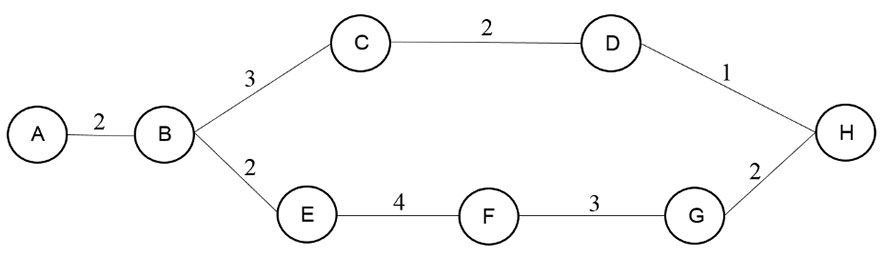
\includegraphics[width=8cm]{item-illustrations/G1-Q10}\par}
	\begin{multicols}{4}\begin{enumerate}[label=\textbf{\Alph*.},align=left,left=1cm..0cm,itemindent=*]
		\item $576$. \item $19$. \item $104$. \item $108$.
	\end{enumerate}\end{multicols}
	\item Để tạo một chiếc bánh phải trải qua 3 giai đoạn. Giai đoạn 1 có thể thực hiện bằng 3 cách, giai đoạn 2 có thể thực hiện bằng 4 cách, giai đoạn 3 có thể thực hiện bằng 1 cách. Vậy để hoàn thành chiếc bánh có tất cả bao nhiêu cách?
	\begin{multicols}{4}\begin{enumerate}[label=\textbf{\Alph*.},align=left,left=1cm..0cm,itemindent=*]
		\item 8 cách. \item 12 cách. \item 3 cách. \item 6 cách.
	\end{enumerate}\end{multicols}
	\item Cho đa giác $n$ đỉnh ($n\in \mathbb{N}^{*},n>3$). Tìm n biết rằng đa giác có 135 đường chéo.
	\begin{multicols}{4}\begin{enumerate}[label=\textbf{\Alph*.},align=left,left=1cm..0cm,itemindent=*]
		\item $15$. \item $27$. \item $8$. \item $18$.
	\end{enumerate}\end{multicols}
	\item Cho $P(A)=\frac 13$, $P(B)=x$, $P(A\cup B)=\frac 12$. Tìm $x$ để $A$ và $B$ xung khắc.
	\begin{multicols}{4}\begin{enumerate}[label=\textbf{\Alph*.},align=left,left=1cm..0cm,itemindent=*]
		\item $x=\frac 17$. \item $x=\frac 16$. \item $x=\frac 18$. \item $x=\frac 15$.
	\end{enumerate}\end{multicols}
	\item Một liên đoàn bóng đá có 10 đội, mỗi đội phải đá 4 trận với đội khác, 2 trận ở sân nhà và 2 trận ở sân khách. Số trận đấu được sắp xếp là
	\begin{multicols}{4}\begin{enumerate}[label=\textbf{\Alph*.},align=left,left=1cm..0cm,itemindent=*]
		\item $180$. \item $160$. \item $90$. \item $45$.
	\end{enumerate}\end{multicols}
	\item Với các chữ số $2$, $3$, $4$, $5$, $6$, có thể lập được bao nhiêu số tự nhiên gồm 5 chữ số khác nhau trong đó hai chữ số $2$ và $3$ không đứng cạnh nhau?
	\begin{multicols}{4}\begin{enumerate}[label=\textbf{\Alph*.},align=left,left=1cm..0cm,itemindent=*]
		\item $120$. \item $96$. \item $72$. \item $48$.
	\end{enumerate}\end{multicols}
	\item Cho hai đường thẳng $d_1$ và $d_2$ song song nhau. Trên $d_1$ lấy 10 điểm phân biệt, trên $d_2$ lấy $n$ điểm phân biệt ($n>3,n\in\mathbb{N}^{*}$). Biết rằng có 2800 tam giác có đỉnh là các điểm đã cho. Tìm $n$.
	\begin{multicols}{4}\begin{enumerate}[label=\textbf{\Alph*.},align=left,left=1cm..0cm,itemindent=*]
		\item $15$. \item $20$. \item $25$. \item $30$.
	\end{enumerate}\end{multicols}
	\item Cho lai hai cá thể có kiểu gen giống nhau là AaBb. Có tất cả bao nhiêu kiểu hình đời $\text{F}_1$?
	\begin{multicols}{4}\begin{enumerate}[label=\textbf{\Alph*.},align=left,left=1cm..0cm,itemindent=*]
		\item 16 kiểu. \item 4 kiểu. \item 2 kiểu. \item 8 kiểu.
	\end{enumerate}\end{multicols}
	\item Cho bất phương trình $C_{n}^{5}<C_{n}^{3}$. Tập nghiệm của bất phương trình đó là
	\begin{enumerate}[label=\textbf{\Alph*.},align=left,left=1cm..0cm,itemindent=*]
		\item $4<n<6$. \item $4<n<7$. \item $5<n<8$. \item $-1<n<8$.
	\end{enumerate}
	\item Một mạch điện có $n$ linh kiện được mắc nối tiếp như hình vẽ sau:\par
	{\centering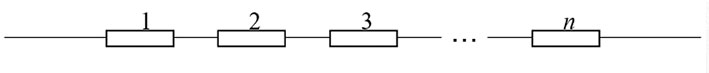
\includegraphics[width=10cm]{item-illustrations/G2-Q17}\par}
	Giả sử các linh kiện có độ tin cậy (xác suất hoạt động tốt) như nhau và bằng $p$. Tính độ tin cậy của mạch điện.
	\begin{multicols}{4}\begin{enumerate}[label=\textbf{\Alph*.},align=left,left=1cm..0cm,itemindent=*]
		\item $p^n$. \item $np$. \item $1-p^n$. \item $1-np$.
	\end{enumerate}\end{multicols}
	\item Có chín tấm thẻ được đánh số từ 1 đến 9. Lần lượt rút thẻ mỗi lần một tấm đến khi được thẻ số 3 thì dừng lại. Phải bóc bao nhiêu lần để xác suất $P\approx 0,088$?
	\begin{multicols}{4}\begin{enumerate}[label=\textbf{\Alph*.},align=left,left=1cm..0cm,itemindent=*]
		\item 3 lần. \item 2 lần. \item 1 lần. \item 4 lần.
	\end{enumerate}\end{multicols}
	\item Xếp ngẫu nhiên 4 người đàn ông, hai người đàn bà và một đứa trẻ vào bảy chiếc ghế đặt quanh một bàn tròn. Tính xác suất để đứa trẻ ngồi giữa hai người đàn bà.
	\begin{multicols}{4}\begin{enumerate}[label=\textbf{\Alph*.},align=left,left=1cm..0cm,itemindent=*]
		\item $\frac{3!3!}{6!}$. \item $\frac{1!2!3!}{6!}$. \item $\frac{2!4!}{6!}$. \item $\frac{1!5!}{6!}$.
	\end{enumerate}\end{multicols}
	\item Gieo đồng thời 3 con xúc xắc. Tính số khả năng tổng số chấm trên mặt xuất hiện của 3 con súc sắc bằng 10.
	\begin{multicols}{4}\begin{enumerate}[label=\textbf{\Alph*.},align=left,left=1cm..0cm,itemindent=*]
		\item $7$. \item $27$. \item $42$. \item $50$.
	\end{enumerate}\end{multicols}
	\item Số các ước nguyên dương của $540$ là
	\begin{multicols}{4}\begin{enumerate}[label=\textbf{\Alph*.},align=left,left=1cm..0cm,itemindent=*]
		\item $12$. \item $23$. \item $24$. \item $36$.
	\end{enumerate}\end{multicols}
	\item Một họ gồm $m$ đường thẳng song song cắt một họ gồm $n$ đường thẳng song song khác ($m,n\geqslant 2$). Có bao nhiêu hình bình hành được tạo thành?
	\begin{enumerate}[label=\textbf{\Alph*.},align=left,left=1cm..0cm,itemindent=*]
		\item $\frac{m(m-1).n(n-1)}{4}$. \item $\frac{m(m-1)+n(n-1)}{2}$. \item $m(m-1).n(n-1)$. \item $m(m-1)+n(n-1)$.
	\end{enumerate}
	\item Ở chó gen lông ngắn kí hiệu là Aa và gen lông dài kí hiệu là aa. Thực hiện phép lai giống chó lông dài và giống chó lông ngắn thu được $\text{F}_1$. Tiếp tục thực hiện lai $\text{F}_1\times \text{F}_1$ thì được đời $\text{F}_2$. Tỉ lệ chó lông ngắn và lông dài ở đời $\text{F}_2$ là bao nhiêu?
	\begin{multicols}{4}\begin{enumerate}[label=\textbf{\Alph*.},align=left,left=1cm..0cm,itemindent=*]
		\item $1:1$. \item $1:5$. \item $5:1$. \item $5:2$.
	\end{enumerate}\end{multicols}
	\item Ba người chơi trò tung xu vào một chiếc bát được đặt trong một chậu nước lớn. Chiếc bát có bán kính 9cm, chiếc chậu có bán kính 50cm. Mỗi người chơi được dùng 3 đồng xu tung đến khi nào có một đồng xu rơi vào bát thì thôi. Số xu trung bình cả ba người sử dụng và độ lệch chuẩn của nó lần lượt.\par
	{\centering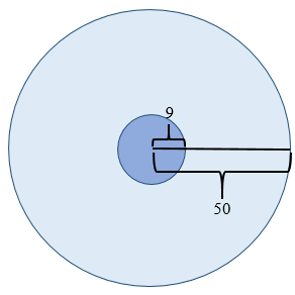
\includegraphics[width=4cm]{item-illustrations/G2-Q96}\par}
	\begin{enumerate}[label=\textbf{\Alph*.},align=left,left=1cm..0cm,itemindent=*]
		\item 2 xu và 0,26. \item 1 xu và 0,26. \item 2 xu và 0,6. \item 1 xu và 0,6.
	\end{enumerate}
\end{enumerate}

\noindent\textbf{Đề thực nghiệm 2:}
\begin{enumerate}[label=\textbf{Câu \arabic*.},align=left,left=0cm..0cm,itemindent=*]
	\item Từ các số $2$, $3$, $4$, $5$ có thể lập được bao nhiêu số gồm 4 chữ số?
	\begin{multicols}{4}\begin{enumerate}[label=\textbf{\Alph*.},align=left,left=1cm..0cm,itemindent=*]
		\item $256$. \item $120$. \item $24$. \item $16$.
	\end{enumerate}\end{multicols}
	\item Có bao nhiêu số tự nhiên gồm 4 chữ số khác nhau?
	\begin{multicols}{4}\begin{enumerate}[label=\textbf{\Alph*.},align=left,left=1cm..0cm,itemindent=*]
		\item $4536$. \item $4^9$. \item $2156$. \item $4530$.
	\end{enumerate}\end{multicols}
	\item Giả sử một công việc có thể được tiến hành theo 2 phương án $A$ và $B$. Phương án $A$ có thể thực hiện bằng $n$ cách, phương án $B$ có thể thực hiện bằng $m$ cách. Khi đó, số cách thực hiện công việc là
	\begin{multicols}{4}\begin{enumerate}[label=\textbf{\Alph*.},align=left,left=1cm..0cm,itemindent=*]
		\item $mn$. \item $m+n$. \item $\frac 12mn$. \item $\frac 12(m+n)$.
	\end{enumerate}\end{multicols}
	\item Xét hai mệnh đề sau đây:\par
	(I) Mỗi hoán vị $n$ phần tử của một tập hợp là một cách sắp xếp các phần tử của tập hợp đó theo một thứ tự nào đó.\par
	(II) Mỗi hoán vị $n$ phần tử của một tập hợp là một chỉnh hợp chập $n$ của $n$ phần tử đó.\par
	Hãy chọn phương án đúng.
	\begin{enumerate}[label=\textbf{\Alph*.},align=left,left=1cm..0cm,itemindent=*]
		\item Chỉ có (I) đúng. \item Chỉ có (II) đúng. \item (I) và (II) đều đúng. \item (I) và (II) đều sai.
	\end{enumerate}
	\item Tỉ số $\frac{(n+3)!}{(n+1)!}$ bằng bao nhiêu?
	\begin{enumerate}[label=\textbf{\Alph*.},align=left,left=1cm..0cm,itemindent=*]
		\item $(n+3)(n+2)$. \item $(n+3)(n+2)(n+1)$. \item $n^2+4n+4$. \item $n+3$.
	\end{enumerate}
	\item Tổng $T=C_n^0+C_n^1+C_n^2+...+C_n^n$ bằng
	\begin{multicols}{4}\begin{enumerate}[label=\textbf{\Alph*.},align=left,left=1cm..0cm,itemindent=*]
		\item $2^n$. \item $2^n-1$. \item $2^n+1$. \item $4^n$.
	\end{enumerate}\end{multicols}
	\item Công thức cộng xác suất $P(A+B)=P(A)+P(B)$ chỉ đúng khi
	\begin{enumerate}[label=\textbf{\Alph*.},align=left,left=1cm..0cm,itemindent=*]
		\item 2 biến cố xung khác và độc lập.
		\item 2 biến cố độc lập.
		\item Hai biến cố xung khắc.
		\item 2 biến cố đối.
	\end{enumerate}
	\item Chọn phát biểu đúng
	\begin{enumerate}[label=\textbf{\Alph*.},align=left,left=1cm..0cm,itemindent=*]
		\item Hai biến cố xung khắc là hai biến cố đối nhau.
		\item Hai biến cố độc lập là có ít nhất một trong hai biến cố xảy ra.
		\item Hai biến cố xung khắc là hai biến cố cùng xảy ra.
		\item Hai biến cố đối nhau là hai biến cố xung khắc.
	\end{enumerate}
	\item Cho các phát biểu sau:\par
	a) Không gian mẫu là tập hợp tất cả các kết quả của phép thử.\par
	b) Biến cố $A$ liên quan đến phép thử $T$ là biến cố mà việc xảy ra hay không xảy ra của $A$ phụ thuộc vào kết quả của $T$.\par
	c) Tập hợp các biến cố thuận lợi cho cho $A$ được gọi là xác suất thuận lợi của $A$.\par
	d) Xác suất của biến cố $A$ được xác định bởi công thức $P(A)=\frac{P(\Omega_A)}{P(\Omega)}$.\par
	e) Xác suất luôn nhỏ hơn 1 và lớn hơn 0.\par
	f) Xác suất của không gian mẫu luôn bằng 1.\par
	Số phát biểu đúng là
	\begin{multicols}{4}\begin{enumerate}[label=\textbf{\Alph*.},align=left,left=1cm..0cm,itemindent=*]
		\item $3$. \item $4$. \item $5$. \item $6$.
	\end{enumerate}\end{multicols}
	\item Có bao nhiêu số tự nhiên có 2 chữ số mà các chữ số hàng chục lớn hơn chữ số hàng đơn vị?
	\begin{multicols}{4}\begin{enumerate}[label=\textbf{\Alph*.},align=left,left=1cm..0cm,itemindent=*]
		\item $40$. \item $45$. \item $50$. \item $55$.
	\end{enumerate}\end{multicols}
	\item Một người vào cửa hàng ăn, người đó chọn thực đơn gồm 1 món ăn trong 5 món, 1 loại quả tráng miệng trong 5 loại quả tráng miệng và một nước uống trong 3 loại nước uống. Có bao nhiêu cách chọn thực đơn?
	\begin{multicols}{4}\begin{enumerate}[label=\textbf{\Alph*.},align=left,left=1cm..0cm,itemindent=*]
		\item $25$. \item $75$. \item $100$. \item $15$.
	\end{enumerate}\end{multicols}
	\item Số các số tự nhiên gồm 5 chữ số chia hết cho 10 là
	\begin{multicols}{4}\begin{enumerate}[label=\textbf{\Alph*.},align=left,left=1cm..0cm,itemindent=*]
		\item $3260$. \item $3168$. \item $9000$. \item $12070$.
	\end{enumerate}\end{multicols}
	\item Số điện thoại ở huyện Củ Chi có 7 chữ số và có 3 chữ số đầu tiên là 790. Hỏi ở huyện Củ Chi có tối đa bao nhiêu máy điện thoại?
	\begin{multicols}{4}\begin{enumerate}[label=\textbf{\Alph*.},align=left,left=1cm..0cm,itemindent=*]
		\item $1000$. \item $100000$. \item $10000$. \item $1000000$.
	\end{enumerate}\end{multicols}
	\item Cho $B=\{1,2,3,4,5,6\}$. Từ tập $B$ có thể lập được bao nhiêu số chẵn có 6 chữ số đôi một khác nhau?
	\begin{multicols}{4}\begin{enumerate}[label=\textbf{\Alph*.},align=left,left=1cm..0cm,itemindent=*]
		\item $720$. \item $46656$. \item $2160$. \item $360$.
	\end{enumerate}\end{multicols}
	\item Thập giác lồi (10 cạnh) là một đa giác có bao nhiêu đường chéo?
	\begin{multicols}{4}\begin{enumerate}[label=\textbf{\Alph*.},align=left,left=1cm..0cm,itemindent=*]
		\item $36$. \item $45$. \item $25$. \item $35$.
	\end{enumerate}\end{multicols}
	\item Trong các khẳng định sau:\par
	a) $P(A)=1$ thì $A$ là biến cố chắc chắn.\par
	b) $A\cap B=\varnothing$ thì $A$ và $B$ là các biến cố đối nhau.\par
	c) $P(B)=0$ thì $B$ là biến cố 0.\par
	d) $A,\overline{A}$ là hai biến cố đối thì $P(A)+P\left(\overline{A}\right)=1$.\par
	e) $A$ và $B$ là hai biến cố bất kỳ thì $P (A\cup B)=P(A)+P(B)-P (A\cap B)$.\par
	Số khẳng định đúng là
	\begin{multicols}{4}\begin{enumerate}[label=\textbf{\Alph*.},align=left,left=1cm..0cm,itemindent=*]
		\item $2$. \item $3$. \item $4$. \item $5$.
	\end{enumerate}\end{multicols}
	\item Gọi $T$ là xác suất sinh con trai, $G$ là xác suất sinh con gái. Khi đó, xác suất sinh toàn con gái là\par
	a) $P=(G)^n,~(n\in\mathbb{N}^*)$.\par
	b) $P=(T)^n,~(n\in\mathbb{N}^*)$.\par
	c) $P=(1-T)^n,~(n\in\mathbb{N}^*)$.\par
	d) $P=1-(T)^n,~(n\in\mathbb{N}^*)$.\par
	Số đáp án đúng là
	\begin{multicols}{4}\begin{enumerate}[label=\textbf{\Alph*.},align=left,left=1cm..0cm,itemindent=*]
		\item $1$. \item $2$. \item $3$. \item $4$.
	\end{enumerate}\end{multicols}
	\item Có bao nhiêu số tự nhiên có 4 chữ số đôi một khác nhau không vượt quá 2020?
	\begin{multicols}{4}\begin{enumerate}[label=\textbf{\Alph*.},align=left,left=1cm..0cm,itemindent=*]
		\item $1008$. \item $1020$. \item $504$. \item $511$.
	\end{enumerate}\end{multicols}
	\item Trong không gian $Oxyz$ cho $n$ điểm trong đó có $m$ điểm đồng phẳng ($1<m\leqslant n$). Có bao nhiêu tứ diện có các đỉnh là các điểm đã cho?
	\begin{enumerate}[label=\textbf{\Alph*.},align=left,left=1cm..0cm,itemindent=*]
		\item $C_{n}^{4}$.
		\item $C_{n}^{4}-C_{n-m}^{4}$.
		\item $C_{n-m}^{4}$.
		\item $C_{n}^{4}-C_{m}^{4}$.
	\end{enumerate}
	\item Tìm số cạnh của một đa giác lồi, biết đa giác có số đường chéo gấp đôi số cạnh.
	\begin{multicols}{4}\begin{enumerate}[label=\textbf{\Alph*.},align=left,left=1cm..0cm,itemindent=*]
		\item $7$. \item $4$. \item $5$. \item $6$.
	\end{enumerate}\end{multicols}
	\item Cho lai cây hoa đỏ cánh dài thuần chủng với cây hoa trắng cánh ngắn thuần chủng được $\text{F}_1$. Có tất cả bao nhiêu kiểu hình của đời $\text{F}_1$?
	\begin{enumerate}[label=\textbf{\Alph*.},align=left,left=1cm..0cm,itemindent=*]
		\item 16 kiểu hình. \item 4 kiểu hình. \item 8 kiểu hình. \item 12 kiểu hình.
	\end{enumerate}
	\item Giải bất phương trình $8C_{105}^{n}<3C_{105}^{n+1}$.
	\begin{enumerate}[label=\textbf{\Alph*.},align=left,left=1cm..0cm,itemindent=*]
		\item $0\leqslant n\leqslant 20$.
		\item $0\leqslant n\leqslant 21$.
		\item $0\leqslant n\leqslant 27$.
		\item $0\leqslant n\leqslant 25$.
	\end{enumerate}
	\item Ba xạ thủ I, II và III cùng bắn (độc lập) mỗi người một viên đạn vào một tấm bia. Xác suất bắn trúng của các xạ thủ lần lượt là 0,7; 0,8; 0,9. Xác suất bia không trúng đạn là
	\begin{multicols}{4}\begin{enumerate}[label=\textbf{\Alph*.},align=left,left=1cm..0cm,itemindent=*]
		\item $0,504$. \item $0,092$. \item $0,587$. \item $0,006$.
	\end{enumerate}\end{multicols}
	\item Trong giải bóng đá của một trường có 12 lớp tham gia, trong đó một đội là của lớp 12A1 và một đội của lớp 12A2. Ban tổ chức tiến hành bốc thăm ngẫu nhiên để phân chia các đội ra thành hai bảng A và B. Tính xác suất để hai đội lớp 12A1 và 12A2 ở cùng một bảng.
	\begin{multicols}{4}\begin{enumerate}[label=\textbf{\Alph*.},align=left,left=1cm..0cm,itemindent=*]
		\item $\frac{5}{11}$. \item $\frac{3}{11}$. \item $\frac{4}{11}$. \item $\frac{2}{11}$.
	\end{enumerate}\end{multicols}
	\item Từ các số $1$, $2$, $3$, $4$ có thể lập được bao nhiêu số tự nhiên có 9 chữ số sao cho các chữ số theo thứ tự từ trái sang phải không giảm và có mặt đủ các chữ số đã cho?
	\begin{multicols}{4}\begin{enumerate}[label=\textbf{\Alph*.},align=left,left=1cm..0cm,itemindent=*]
		\item 56 số. \item 60 số. \item 58 số. \item 62 số.
	\end{enumerate}\end{multicols}
	\item Từ các số $1$, $2$, $3$, $4$, $5$, $6$, $7$ có thể lập được bao nhiêu số có 5 chữ số nhỏ hơn $30000$?
	\begin{multicols}{4}\begin{enumerate}[label=\textbf{\Alph*.},align=left,left=1cm..0cm,itemindent=*]
		\item $360$. \item $720$. \item $1080$. \item $920$.
	\end{enumerate}\end{multicols}
	\item Cho 10 điểm $A_1, A_2, A_3,..., A_{10}$, trong đó có 4 điểm thẳng hàng ngoài ra không có 3 điểm nào khác thẳng hàng. Hỏi có bao nhiêu tam giác có 3 đỉnh là 3 điểm trong 10 điểm đã cho?
	\begin{enumerate}[label=\textbf{\Alph*.},align=left,left=1cm..0cm,itemindent=*]
		\item 80 tam giác. \item 96 tam giác. \item 60 tam giác. \item 116 tam giác.
	\end{enumerate}
	\item Có một mạch điện như sau:\par
	{\centering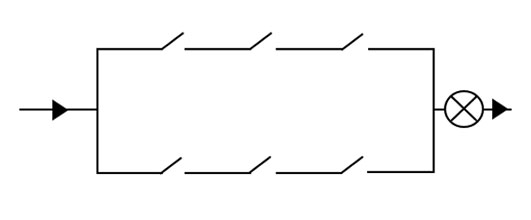
\includegraphics[width=9cm]{item-illustrations/G1-Q39}\par}
	Có bao nhiêu cách bật công tắc để làm sáng bóng đèn?
	\begin{multicols}{4}\begin{enumerate}[label=\textbf{\Alph*.},align=left,left=1cm..0cm,itemindent=*]
		\item 3 cách. \item 6 cách. \item $3!$ cách. \item $6!$ cách.
	\end{enumerate}\end{multicols}
	\item Ở đậu Hà lan, tính trạng hạt màu vàng trội hoàn toàn so với tính trạng hạt màu xanh. Tính trạng do một gen qui định nằm ở NST thường. Cho 5 cây tự thụ và sau khi thu hoạch lấy ngẫu nhiên mỗi cây một hạt đem gieo được các cây $\text{F}_1$. Xác suất để trong 5 cây có 3 cây cho hạt vàng và 2 cây cho hạt xanh.
	\begin{enumerate}[label=\textbf{\Alph*.},align=left,left=1cm..0cm,itemindent=*]
		\item $P=0,026$. \item $P=0,088$. \item $P=0,264$. \item $P=0,274$.
	\end{enumerate}
	\item Xác suất trúng một viên đạn vào mục tiêu là 0,8. Thực hiện bắn vào mục tiêu trong điều kiện như nhau cho đến khi có 5 viên trúng mục tiêu thì dừng. gọi $X$ là số đạn cần bắn. Tìm phân phối xác suất của $X$.
	\begin{enumerate}[label=\textbf{\Alph*.},align=left,left=1cm..0cm,itemindent=*]
		\item $P\left[ X=k+i \right]=C_{k+i-1}^{k-1}.{{p}^{k}}.{{\left( 1-p \right)}^{i}}$.
		\item $P\left[ X=k+i \right]=C_{k+i}^{k}.{{p}^{k}}.{{\left( 1-p \right)}^{i}}$.
		\item $P\left[ X=k+i \right]=C_{k+i-1}^{k-1}.{{p}^{i}}.{{\left( 1-p \right)}^{k}}$.
		\item $P\left[ X=k+i \right]=C_{k+i}^{k}.{{p}^{i}}.{{\left( 1-p \right)}^{k}}$.
	\end{enumerate}
\end{enumerate}

\noindent\textbf{Đáp án đề thực nghiệm}
\begin{longtable}{ScScScScSc}
	\textbf{Câu hỏi} & \textbf{Mức độ} & \textbf{Đáp án} & \textbf{Mức độ} & \textbf{Đáp án}\\\hline
	& \multicolumn{2}{Sc}{\textbf{Đề 1}} & \multicolumn{2}{Sc}{\textbf{Đề 2}}\\\hline\endhead\hline\endfoot
	Câu 1  & 1 & A & 1 & A \\
	Câu 2  & 1 & A & 1 & A \\
	Câu 3  & 1 & C & 1 & B \\
	Câu 4  & 1 & B & 1 & C \\
	Câu 5  & 1 & C & 1 & A \\
	Câu 6  & 1 & B & 1 & A \\
	Câu 7  & 1 & B & 1 & C \\
	Câu 8  & 1 & B & 1 & B \\
	Câu 9  & 1 & A & 1 & A \\
	Câu 10 & 1 & B & 2 & B \\
	Câu 11 & 2 & D & 2 & B \\
	Câu 12 & 2 & D & 2 & C \\
	Câu 13 & 2 & A & 2 & C \\
	Câu 14 & 2 & D & 2 & D \\
	Câu 15 & 2 & B & 2 & D \\
	Câu 16 & 2 & D & 2 & C \\
	Câu 17 & 2 & B & 2 & B \\
	Câu 18 & 3 & A & 3 & D \\
	Câu 19 & 3 & C & 3 & D \\
	Câu 20 & 3 & B & 3 & A \\
	Câu 21 & 3 & B & 3 & B \\
	Câu 22 & 3 & D & 3 & B \\
	Câu 23 & 3 & A & 3 & D \\
	Câu 24 & 3 & A & 3 & C \\
	Câu 25 & 3 & D & 4 & D \\
	Câu 26 & 3 & B & 4 & B \\
	Câu 27 & 3 & C & 4 & D \\
	Câu 28 & 4 & A & 4 & A \\
	Câu 29 & 4 & D & 4 & A \\
	Câu 30 & 4 & A & 4 & B \\
\end{longtable}

02 đề thực nghiệm trên được thực nghiệm với 120 học sinh thuộc các trường THPT trên địa bàn Cần Thơ: THPT An Khánh, THPT Bùi Hữu Nghĩa, THPT Châu Văn Liêm, THPT chuyên Lý Tự Trọng, THPT Nguyễn Việt Hồng, THPT Thực hành Sư phạm (Đại học Cần Thơ). Sau khi phân tích bằng phần mềm IATA, thu được số liệu ở bảng \ref{tab:tab-s2-1-iata}.

\begin{longtable}{SlSrSrSrSrSrSrSc}
	\caption{Kết quả phân tích đề thực nghiệm qua phần mềm IATA} \label{tab:tab-s2-1-iata} \\
	\multicolumn{1}{Sc}{\textbf{Câu hỏi}} & \multicolumn{1}{Sc}{\textbf{Discr}} & \multicolumn{1}{Sc}{\textbf{PVal}} & \multicolumn{1}{Sc}{\textbf{PBis}} & \multicolumn{1}{Sc}{\textbf{$a$}} & \multicolumn{1}{Sc}{\textbf{$b$}} & \multicolumn{1}{Sc}{\textbf{$c$}} & \textbf{Ghi chú}\\\hline\endfirsthead

	\multicolumn{1}{Sc}{\textbf{Câu hỏi}} & \multicolumn{1}{Sc}{\textbf{Discr}} & \multicolumn{1}{Sc}{\textbf{PVal}} & \multicolumn{1}{Sc}{\textbf{PBis}} & \multicolumn{1}{Sc}{\textbf{$a$}} & \multicolumn{1}{Sc}{\textbf{$b$}} & \multicolumn{1}{Sc}{\textbf{$c$}} & \textbf{Ghi chú}\\\hline\endhead\hline\endfoot

	\multicolumn{8}{Sc}{\textbf{Đề 1}} \\\hline
	Câu 1  & $0.10$  & $0.96$ & $0.38$  & $1.24$  & $-2.43$  & $0$ &      \\
	Câu 2  & $0.15$  & $0.91$ & $0.33$  & $0.74$  & $-2.31$  & $0$ &      \\
	Câu 3  & $-0.13$ & $0.08$ & $-0.12$ & $-0.43$ & $-3.67$  & $0$ & Loại \\
	Câu 4  & $0.44$  & $0.56$ & $0.26$  & $0.25$  & $-0.56$  & $0$ &      \\
	Câu 5  & $0.35$  & $0.82$ & $0.36$  & $0.63$  & $-1.73$  & $0$ &      \\
	Câu 6  & $0.25$  & $0.35$ & $0.23$  & $0.15$  & $2.59$   & $0$ &      \\
	Câu 7  & $0.53$  & $0.75$ & $0.55$  & $1.62$  & $-0.79$  & $0$ &      \\
	Câu 8  & $-0.03$ & $0.01$ & $-0.37$ & $-2.26$ & $-2.92$  & $0$ & Loại \\
	Câu 9  & $0.36$  & $0.30$ & $0.30$  & $0.27$  & $1.92$   & $0$ &      \\
	Câu 10 & $0.58$  & $0.78$ & $0.53$  & $1.27$  & $-0.98$  & $0$ &      \\
	Câu 11 & $0.19$  & $0.92$ & $0.39$  & $0.78$  & $-2.35$  & $0$ &      \\
	Câu 12 & $0.29$  & $0.89$ & $0.42$  & $1.42$  & $-1.56$  & $0$ &      \\
	Câu 13 & $0.39$  & $0.84$ & $0.47$  & $1.06$  & $-1.38$  & $0$ &      \\
	Câu 14 & $0.35$  & $0.72$ & $0.27$  & $0.35$  & $-1.68$  & $0$ &      \\
	Câu 15 & $0.45$  & $0.84$ & $0.54$  & $1.62$  & $-1.18$  & $0$ &      \\
	Câu 16 & $0.41$  & $0.84$ & $0.55$  & $1.58$  & $-1.19$  & $0$ &      \\
	Câu 17 & $0.45$  & $0.87$ & $0.49$  & $1.15$  & $-1.50$  & $0$ &      \\
	Câu 18 & $0.35$  & $0.82$ & $0.38$  & $0.33$  & $-2.92$  & $0$ &      \\
	Câu 19 & $0.32$  & $0.86$ & $0.29$  & $0.28$  & $-3.93$  & $0$ &      \\
	Câu 20 & $0.26$  & $0.85$ & $0.45$  & $0.58$  & $-2.08$  & $0$ &      \\
	Câu 21 & $0.52$  & $0.45$ & $0.36$  & $0.48$  & $0.27$   & $0$ &      \\
	Câu 22 & $0.46$  & $0.31$ & $0.30$  & $0.56$  & $1.00$   & $0$ &      \\
	Câu 23 & $0.58$  & $0.51$ & $0.44$  & $0.95$  & $-0.05$  & $0$ &      \\
	Câu 24 & $0.03$  & $0.37$ & $0.06$  & $-0.21$ & $-1.52$  & $0$ & Loại \\
	Câu 25 & $-0.06$ & $0.06$ & $-0.14$ & $-0.29$ & $-5.81$  & $0$ & Loại \\
	Câu 26 & $0.04$  & $0.65$ & $0.06$  & $-0.15$ & $2.40$   & $0$ & Loại \\
	Câu 27 & $0.31$  & $0.85$ & $0.43$  & $0.71$  & $-1.80$  & $0$ &      \\
	Câu 28 & $0.41$  & $0.77$ & $0.38$  & $0.79$  & $-1.19$  & $0$ &      \\
	Câu 29 & $-0.08$ & $0.22$ & $0.06$  & $-0.19$ & $-3.94$  & $0$ & Loại \\
	Câu 30 & $0.04$  & $0.31$ & $0.06$  & $-0.04$ & $-12.62$ & $0$ & Loại \\\hline
	\multicolumn{8}{Sc}{\textbf{Đề 2}} \\\hline
	Câu 1  & $0.12$  & $0.89$ & $0.09$  & $-0.08$ & $15.91$  & $0$ & Loại \\
	Câu 2  & $0.04$  & $0.99$ & $0.21$  & $1.05$  & $-3.50$  & $0$ &      \\
	Câu 3  & $0.16$  & $0.86$ & $0.36$  & $0.79$  & $-1.75$  & $0$ &      \\
	Câu 4  & $0.34$  & $0.44$ & $0.32$  & $0.37$  & $0.43$   & $0$ &      \\
	Câu 5  & $0.12$  & $0.93$ & $0.34$  & $0.79$  & $-2.45$  & $0$ &      \\
	Câu 6  & $0.44$  & $0.85$ & $0.42$  & $1.01$  & $-1.48$  & $0$ &      \\
	Câu 7  & $0.33$  & $0.69$ & $0.35$  & $0.51$  & $-1.09$  & $0$ &      \\
	Câu 8  & $0.11$  & $0.17$ & \multicolumn{1}{Sc}{$-$} & $-0.03$ & $-29.74$ & $0$ & Loại \\
	Câu 9  & $0.23$  & $0.18$ & $0.17$  & $0.20$  & $4.69$   & $0$ &      \\
	Câu 10 & $0.04$  & $0.96$ & $0.02$  & $-0.43$ & $4.55$   & $0$ & Loại \\
	Câu 11 & $0.20$  & $0.96$ & $0.43$  & $1.29$  & $-2.26$  & $0$ &      \\
	Câu 12 & $0.08$  & $0.98$ & $0.51$  & $2.50$  & $-2.59$  & $0$ &      \\
	Câu 13 & $0.16$  & $0.91$ & $0.38$  & $1.09$  & $-1.89$  & $0$ &      \\
	Câu 14 & $0.32$  & $0.70$ & $0.35$  & $0.22$  & $-2.33$  & $0$ &      \\
	Câu 15 & $0.28$  & $0.88$ & $0.43$  & $0.72$  & $-2.01$  & $0$ &      \\
	Câu 16 & $0.34$  & $0.37$ & $0.26$  & $0.06$  & $5.00$   & $0$ &      \\
	Câu 17 & $0.17$  & $0.72$ & $0.17$  & $0.01$  & $-59.17$ & $0$ &      \\
	Câu 18 & $0.44$  & $0.82$ & $0.48$  & $1.06$  & $-1.24$  & $0$ &      \\
	Câu 19 & $0.46$  & $0.35$ & $0.38$  & $1.44$  & $0.46$   & $0$ &      \\
	Câu 20 & $0.48$  & $0.86$ & $0.57$  & $1.37$  & $-1.36$  & $0$ &      \\
	Câu 21 & $0.12$  & $0.74$ & $0.02$  & $-0.05$ & $11.37$  & $0$ & Loại \\
	Câu 22 & $-0.16$ & $0.11$ & $-0.11$ & $-0.3$  & $-4.20$  & $0$ & Loại \\
	Câu 23 & $0.28$  & $0.84$ & $0.42$  & $0.74$  & $-1.70$  & $0$ &      \\
	Câu 24 & $-0.04$ & $0.04$ & $-0.15$ & $-0.38$ & $-5.05$  & $0$ & Loại \\
	Câu 25 & $0.08$  & $0.06$ & $0.16$  & $-0.05$ & $-30.08$ & $0$ & Loại \\
	Câu 26 & $0.48$  & $0.68$ & $0.32$  & $0.57$  & $-0.90$  & $0$ &      \\
	Câu 27 & $0.36$  & $0.80$ & $0.42$  & $0.56$  & $-1.69$  & $0$ &      \\
	Câu 28 & $0.14$  & $0.40$ & $0.05$  & $-0.01$ & $-27.39$ & $0$ & Loại \\
	Câu 29 & $0.26$  & $0.32$ & $0.04$  & $-0.17$ & $-2.55$  & $0$ & Loại \\
	Câu 30 & $0.14$  & $0.32$ & $0.05$  & $-0.10$ & $-4.47$  & $0$ & Loại \\
\end{longtable}

Đến đây, ngân hàng câu hỏi chương Tổ hợp – Xác suất được tổng hợp và chuẩn hóa gồm 87 câu hỏi thuộc 04 chủ đề. Tuy nhiên, các câu hỏi thuộc chủ đề \textit{Quy tắc đếm} có \textit{độ khó} ($b$) và \textit{độ phân biệt} rất thấp, cụ thể phần lớn câu hỏi có $b<0$ nên không thể dùng để đánh giá như một chủ đề riêng lẽ. Do đó, chủ đề \textit{Quy tắc đếm} được gộp chung với \textit{HV, TH, CH}. Số lượng các câu hỏi của ngân hàng câu hỏi được tổng hợp trong bảng \ref{tab:tab-s2-2-stats}.\par

\begin{longtable}{SlScScScScSc}
	\caption{Số lượng câu hỏi của ngân hàng câu hỏi chương Tổ hợp – Xác suất} \label{tab:tab-s2-2-stats}\\
	\multicolumn{1}{Sc}{\textbf{Chủ đề}} & \textbf{Mức độ 1} & \textbf{Mức độ 2} & \textbf{Mức độ 3} & \textbf{Mức độ 4} & \textbf{Tổng cộng}\\\hline\endfirsthead

	\multicolumn{1}{Sc}{\textbf{Chủ đề}} & \textbf{Mức độ 1} & \textbf{Mức độ 2} & \textbf{Mức độ 3} & \textbf{Mức độ 4} & \textbf{Tổng cộng}\\\hline\endhead\hline\endfoot

	Quy tắc đếm     & $5$ & $9$  & $7$ & $1$ & $22$ \\
	HV, TH, CH      & $6$ & $6$  & $6$ & $2$ & $20$ \\
	Nhị thức Newton & $7$ & $7$  & $9$ & $2$ & $25$ \\
	Xác suất        & $5$ & $10$ & $4$ & $1$ & $20$ \\
	\textbf{Tổng cộng} & $23$ & $32$ & $26$ & $6$ & $87$ \\
\end{longtable}\par

\section{Xây dựng API trắc nghiệm thích ứng}
\textit{Trắc nghiệm thích ứng} (Adaptive Test) là thuật ngữ để chỉ một phương pháp đánh giá TS (học sinh, sinh viên, bệnh nhân...) bằng hình thức kiểm tra trắc nghiệm nhưng đánh giá theo hướng năng lực của TS bằng bộ CH tương ứng với mức năng lực đó. API trắc nghiệm thích ứng là một hệ thống phần mềm được phát triển trên cơ sở mô hình trắc nghiệm thích ứng để đánh giá TS. Về hoạt động, hệ thống cố gắng mô phỏng phương pháp đánh giá của một người giáo viên đối với học sinh\cite{le2019phat}. Có nghĩa là: lần đầu tiên hệ thống cung cấp cho TS một CH vừa đủ khó đối với TS, nếu TS trả lời chính xác thì sau đó một CH khó hơn sẽ được đề nghị và ngược lại, một CH có độ khó thấp hơn được đề nghị nếu TS trả lời sai. Bên cạnh đó, CH kế tiếp được đề nghị dựa trên dữ liệu trả lời những CH trước đó. Quá trình này được lặp đi lặp lại cho đến khi có đủ bằng chứng để xác định năng lực của TS.\par

\subsection{Thuật toán trắc nghiệm thích ứng}
\subsubsection{Mô tả thuật toán}

\noindent Đầu vào:\par
\begin{itemize}
	\item Ngân hàng câu hỏi đã được chuẩn hóa theo mô hình IRT 2 tham số.
	\item Năng lực hiện tại của thí sinh.
\end{itemize}\par
\noindent Đầu ra: Năng lực của thí sinh sau khi được đánh giá.\par
\noindent Hoạt động thuật toán:\par
\begin{enumerate}[label=\textbf{Bước \arabic*.},align=left,left=0cm..0cm,itemindent=*]
	\item Khởi tạo mức năng lực ban đầu cho TS: $\theta_1=0$.
	\item CH phù hợp với mức năng lực của TS được đưa ra và TS trả lời.
	\item Ước lượng mức độ năng lực mới dựa trên kết quả trả lời CH của TS:
	\begin{equation}\label{eqn:eqn-s2-new-theta}
		\theta_{k+1}=\theta_k+\gamma\sum_{i=1}^{k}\left(u_i-\frac{\mathbf{e}^{a_i(\theta-b_i)}}{1+\mathbf{e}^{a_i(\theta-b_i)}}\right),
	\end{equation}
	với $\gamma=1.0$ là tốc độ học của máy, $u_i=0|1$ là kết quả trả lời CH thứ $i$ của TS, $a_i$, $b_i$ là các tham số của CH.
	\item Quay lại \textbf{Bước 2} nếu các điều kiện dừng chưa được thỏa mãn.
	\item Kết thúc quá trình đánh giá và đưa ra kết quả.
\end{enumerate}\par
Trong đó, \textit{điều kiện dừng} của thuật toán là tất cả CH trong ngân hàng CH đã được trả lời, hoặc hệ số năng lực $\theta$ đã được xác định. Cụ thể, hệ số năng lực được xác định khi độ lệch chuẩn $SE$ đạt giá trị đủ nhỏ, thường là $0.4$ hoặc $0.8$, theo lý thuyết IRT, ta có:
\begin{equation}\label{eqn:eqn-s2-se-theta}
	SE(\theta_k)=\frac{1}{\sqrt{\sum_{i=1}^{k}I_i(\theta_k)}}.
\end{equation}
Hàm thông tin CH trả về giá trị kỳ vọng thay đổi của năng lực. Hay nói cách khác, CH thứ $i$ đã đóng góp thế nào cho sự thay đổi của tham số năng lực. Do đó ta có thể sử dụng như một điều kiện dừng của trắc nghiệm thích ứng.\par

\subsection{Thuật toán lựa chọn câu hỏi}
Thuật toán lựa chọn CH tiếp theo là phần quan trọng nhất trong mô hình trắc nghiệm thích ứng. Đây là một thuật toán con hoạt động bên trong thuật toán trắc nghiệm thích ứng. Thuật toán này giúp máy tính lựa chọn ra CH phù hợp với năng lực thí sinh từ ngân hàng CH đã chuẩn hóa. Cho đến hiện nay, tồn tại các thuật toán lựa chọn CH như sau \cite{tran2017ung}:
\begin{itemize}
	\item Thuật toán lựa chọn CH theo tiêu chuẩn thông tin tối đa (MI) là thuật toán phổ biến được sử dụng trong các mô hình trắc nghiệm thích nghi. CH thứ $k+1$ được lựa chọn cho TS là câu hỏi cung cấp thông tin tối đa cho việc ước lượng khả năng ($\theta_k$) của TS dựa trên $k$ câu hỏi trước đó mà TS đã trả lời.
	\item Thuật toán lựa chọn câu hỏi theo thông tin toàn cục (KL) là thuật toán lựa chọn câu hỏi dựa trên phương pháp thông tin tổng thể. Thuật toán này sử dụng độ đo Kullback – Leibler để tính toán ước lượng trong việc lựa chọn câu hỏi.
	\item Thuật toán lựa chọn câu hỏi dựa trên sự phân tích tiên đoán theo tiêu chí tối đa thông tin (MEI) là thuật toán lựa chọn câu hỏi dựa trên việc phân tích tiên đoán các tiêu chí tối đa thông tin dự kiến.
\end{itemize}\par

\subsubsection{Tiêu chí chọn CH}
Sau khi TS trả lời CH $k$ thì năng lực tạm thời của TS được ước lượng và ký hiệu là $\theta_{k}$. Tiếp theo ta tìm CH thứ $k$ phù hợp với mức năng lực này bằng phương pháp lựa chọn CH theo \textit{tiêu chuẩn thông tin tối đa} (maximum information criterion):
$$i_{k+1}=\mathrm{argmax}_j\left\{I_j\left(\theta_k\right),~j\in R_k\right\}$$
Với $R_k=\left\{1...n\right\}\setminus S_k$, và $S_k={i_1, i_2, ..., i_k}$ là tập hợp CH đã được chọn, $I_j(\theta)$ là hàm thông tin của CH thứ $j$, đối với mô hình IRT 2 tham số, ta có:
$$I_j(\theta)=a_j^2P_j(\theta)Q_j(\theta).$$
Khi $\theta$ cố định, hàm thông tin đạt giá trị cực đại tại điểm $b=0$. Vì vậy câu $i_{k+1}$ được chọn là CH có độ khó gần với $\theta_k$. Nói cách khác, khi giá trị độ khó $b$ càng tiến về giá trị năng lực $\theta$ và độ phân biệt $a$ càng lớn thì hàm thông tin càng tiến gần giá trị cực đại. Do đó, CH thứ $k+1$ được chọn là CH có độ khó gần bằng năng lực ước lượng $\theta_k$ và có độ phân biệt lớn nhất trong ngân hàng.\par

\subsubsection{Thuật toán tìm kiếm nhị phân}
Với bài toán tìm kiếm một giá trị gần nhất với $a$ từ tập hợp $\left\{b_1,b_2,...,b_n\right\}$. \textit{Thuật toán tìm kiếm nhị phân} (binary search algorithm) cho phép ta tìm kiếm một cách tối ưu với độ phức tạp $\mathrm{O}\left(\log_n\right)$: Nếu $a$ nhỏ hơn giá trị trung tâm thì ta tìm kiếm trong nửa trái của dãy, ngược lại thì tìm kiếm trogn nửa phải của dãy, quá trình tiếp tục cho tới khi tìm được giá trị xấp xỉ với $a$.\par
\noindent Đầu vào: $a$ và dãy $\left\{b_1,b_2,...,b_n\right\}$.\par
\noindent Đầu ra: $b$ gần nhất với $a$.\par
\noindent Hoạt động của thuật toán:\par
\begin{enumerate}[label=\textbf{Bước \arabic*.},align=left,left=0cm..0cm,itemindent=*]
	\item Gán $l=1$ và $r=n$.
	\item Nếu $l\geqslant r$, chuyển tới \textbf{Bước 6}.
	\item Gán $m=\left\lfloor\frac{l+r}{2}\right\rfloor$.
	\item Nếu $a=b_m$, tìm kiếm kết thúc và trả về $m$.
	\item Nếu $a<b_m$, gán $r=m-1$, ngược lại, gán $l=m+1$, quay lại \textbf{Bước 2}.
	\item Nếu $|a-b_l|<|a-b_r|$, trả về $l$, ngược lại, trả về $r$. Tìm kiếm kết thúc.
\end{enumerate}
\noindent Code minh họa thuật toán trên ngôn ngữ PHP:
\begin{lstlisting}[language=php,caption=Phương thức tìm kiếm nhị phân]
function binary_search (Int $a, Array $b): Int {
	if (count($b) == 0) return -1;
	$left = 0; $right = count($b) - 1;
	while ($left <= $right) {
		$mid = floor(($left + $right) / 2);
		if ($a == $b[$mid$]) return $mid;
		if ($a < $b[$mid]) $right = $mid - 1; else $left = $mid + 1;
	}
	if (abs($a - $b[$left]) < abs($a - $b[$right])) return $left;
	return $right;
}
\end{lstlisting}
\subsection{Xây dựng API xử lý bằng ngôn ngữ PHP}
Bằng ngôn ngữ web PHP, luận văn tiến hành xây dựng một \textit{không gian tên} (namespace) xử lý dữ liệu CH và bài kiểm tra dựa trên lý thuyết IRT. Trong đó có 02 \textit{lớp} (class) là \texttt{item} và \texttt{test}.
\subsubsection{Class câu hỏi}
Trong class câu hỏi, có hai tham số chính, là $a$ (độ phân biệt) và $b$ (độ khó) cần được khởi tạo ngay từ đầu. Bên cạnh đó, lớp cần cung cấp các phương thức tính xác suất trả lời đúng ($P$), xác suất trả lời sai ($Q=1-P$) và tính hàm lượng thông tin cho việc đánh giá năng lực ($I$).\par
\noindent Code minh họa:
\begin{lstlisting}[language=php,caption=Class câu hỏi]
namespace IRT;
class Item {
	public $a = 0;
	public $b = 0;

	function __construct (Float $a, Float $b) {
		$this -> set_parameter($a, $b);
	}
	function set_parameter (Float $a, Float $b) {
		$this -> a = $a;
		$this -> b = $b;
	}
	function P (Float $theta): Float {
		$exp = exp(($this -> a) * ($theta - ($this -> b)));
		return $exp / (1 + $exp);
	}
	function Q (Float $theta): Float {
		return $this -> P($theta);
	}
	function I (Float $theta): Float {
		$P = $this -> P($theta);
		return $this -> a ** 2 * $P * (1 - $P);
	}
}
\end{lstlisting}

\subsubsection{Class bài kiểm tra}
Class bài kiểm tra bao gồm hai thuộc tính chính là \textit{các câu hỏi} (items) và tốc độ học $\gamma$ của kiểm tra thích ứng. Các phương thức xử lý cần thiết là: Thêm câu hỏi (\texttt{add\_item(item:)} và \texttt{add\_items(items:)}), lấy câu hỏi (\texttt{get\_item(index:)}), xóa câu hỏi (\texttt{remove\_item(index:)}), đếm số câu hỏi (\texttt{num\_of\_items(:)}).\par
Bên cạnh đó, clas cần cung cấp đầy đủ các phương thức tính toán dựa trên lý thuyết IRT, như là: hàm thông tin của đề trắc nghiệm ($I(\theta)$), độ lệch chuẩn $SE(\theta)$ và điểm IRT. Hơn nữa, để phục vụ cho trắc nghiệm thích ứng, một phương thức không thể thiếu là tìm kiếm câu hỏi bằng thuật toán nhị phân (\texttt{binary\_search\_item(theta:)}).\par
\noindent Code minh họa:

\begin{lstlisting}[language=php,caption=Class bài kiểm tra]
namespace IRT;
class Test {
	public $items;
	public $gamma = 1.0;

	function __construct (Array $items = []) {
		$this -> items = $items;
	}
	function add_item (Item $item) {
		array_push($this -> items, $item);
	}
	function add_items (Array $items) {
		$this -> items = array_merge($this -> items, $items);
	}
	function get_item (Int $index): Item {
		return $this -> items[$index];
	}
	function remove_item (Int $index) {
		array_splice($this -> items, $index, 1);
	}
	function num_of_items (): Int {
		return count($this -> items);
	}

	function d_theta (Float $theta, Array $answers): Float {
		$numerator = 0;
		$denominator = 0.000001;
		for ($i = 0, $count = count($answers); $i < $count; $i++) {
			$numerator   += ($this -> items[$i] -> a) * ($answers[$i] - ($this -> items[$i] -> P($theta)));
			$denominator += $this -> items[$i] -> I($theta);
		}
		return $numerator / $denominator;
	}
	function I (Float $theta): Float {
		$sumI = 0.000001;
		for ($i = 0, $count = count($this -> items); $i < $count; $i++)
			$sumI += $this -> items[$i] -> I($theta);
		return $sumI;
	}
	function standard_deviation_expected ($theta): Float {
		return 1 / sqrt($this -> I($theta));
	}
	function IRT (Array $answers, Float $start_theta = 1.0): Array {
		$theta = $start_theta;
		$d_theta = 1.0;
		$d_theta_max = 0.00001;
		$step = 0;
		while ((abs($d_theta) > $d_theta_max) && ($step < 100)) {
			$step++;
			$d_theta = $this -> d_theta($theta, $answers, $this -> items);
			$theta += $d_theta;
		}
		$SumP = 0;
		for ($i = 0, $count = count($answers); $i < $count; $i++)
			$SumP += P($theta, $this -> items[$i]);
		return [
			'step' => $step,
			'theta' => $theta,
			'IRT_score' => $SumP / count($answers)
		];
	}
	function binary_search_item (Float $theta): Int {
		$count = count($this -> items);
		if ($count == 0) return false;
		$low = 0; $high = $count - 1;
		while ($low <= $high) {
			$mid = floor(($low + $high) / 2);
			if ($theta == ($this -> items[$mid] -> b)) return $mid;
			if ($theta < ($this -> items[$mid] -> b)) $high = $mid - 1;
			else $low = $mid + 1;
		}
		if (abs($theta - ($this -> items[$low] -> b)) < abs($theta - ($this -> items[$high] -> b)))
			return $low;
		return $high;
	}
}
\end{lstlisting}
